
Talk about the problem setup, code blocks shown.

\begin{python}
"""
Set up and solve problem with identity map
"""
# import libraries
import bet.sample as sample
import bet.sampling.basicSampling as bsam
import numpy as np
import scipy.stats as sstats

# define input space parameters and model to instantiate sampler object
dimension = 2
numSamples = 100
I = np.eye(dimension)
def model(input_samples):
        return (I@input_samples.T).T
sampler = bsam.sampler(model)

# instantiate objects that hold input/output samples
input_set = bsam.random_sample_set('r', dimension, num_samples=numSamples)
disc = sampler.compute_QoI_and_create_discretization(input_set)

# define inverse problem

# compare with higher-fidelity discretization of output space

\end{python}

Note that there is no need to explictly call {\tt disc.compute\_pushforward()}, (or \pythoninline{disc.compute_predicted()}) since it is computed automatically if none have been previously constructed.
When \pythoninline{disc.updated_pdf()} is called, densities are evaluated at the initial set of $\nsamps$ random samples, and stored in \pythoninline{disc._input_sample_set._densities}.
However, the function \pythoninline{disc.predicted_pdf()} is capable of evaluating the solution at any new set of samples (provided a model is available/equipped to the discretization), something we leverage for plotting on a regular grid.

Once our four discretization objects \pythoninline{disc}, \pythoninline{disc_a}, \pythoninline{disc_b} and \pythoninline{disc_c} have been generated, we can use some utility plotting functions to compare the densities:

\begin{python}
"""
Plotting code to generate figures.
"""
# define plotting parameters
nbins = 50
xmn, xmx = 0.25, 0.75
ymn, ymx = 0.25, 0.75
xi, yi = np.mgrid[xmn:xmx:nbins*1j, ymn:ymx:nbins*1j]

# plotting functions computes nearest-neighbors to
# the regular grid of samples.
plot_2d_comparison(xi, yi, disc_1, disc_2,
                   '$M=1, N=%d$'%(numSamples),
                   '$M=4, N=%d$'%(numSamples))
\end{python}

\begin{figure}[ht]
\begin{minipage}{.975\textwidth}
  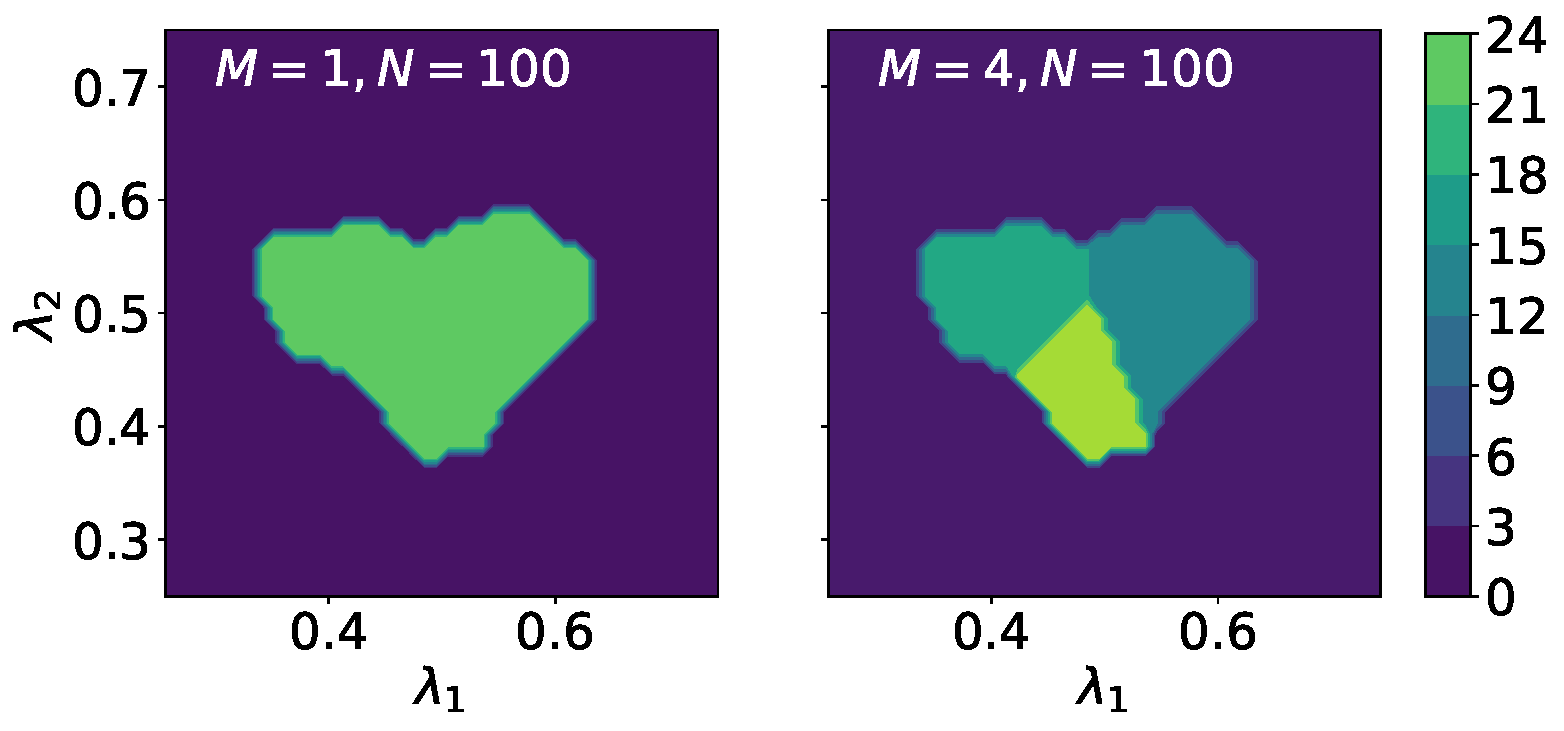
\includegraphics[width=\linewidth]{./examples/identity/set/M1-N100_N100-vs-M4-N100_N100.pdf}
\end{minipage}
\caption{
$\nsamps=100$ were used to discretize $\pspace$ and $\ndiscs=1, 4$ (left/right) were used to discretize $\dspace$.
TK
}
\label{fig:ex:identity_set_1E2}
\end{figure}

\begin{figure}[ht]
\begin{minipage}{.975\textwidth}
  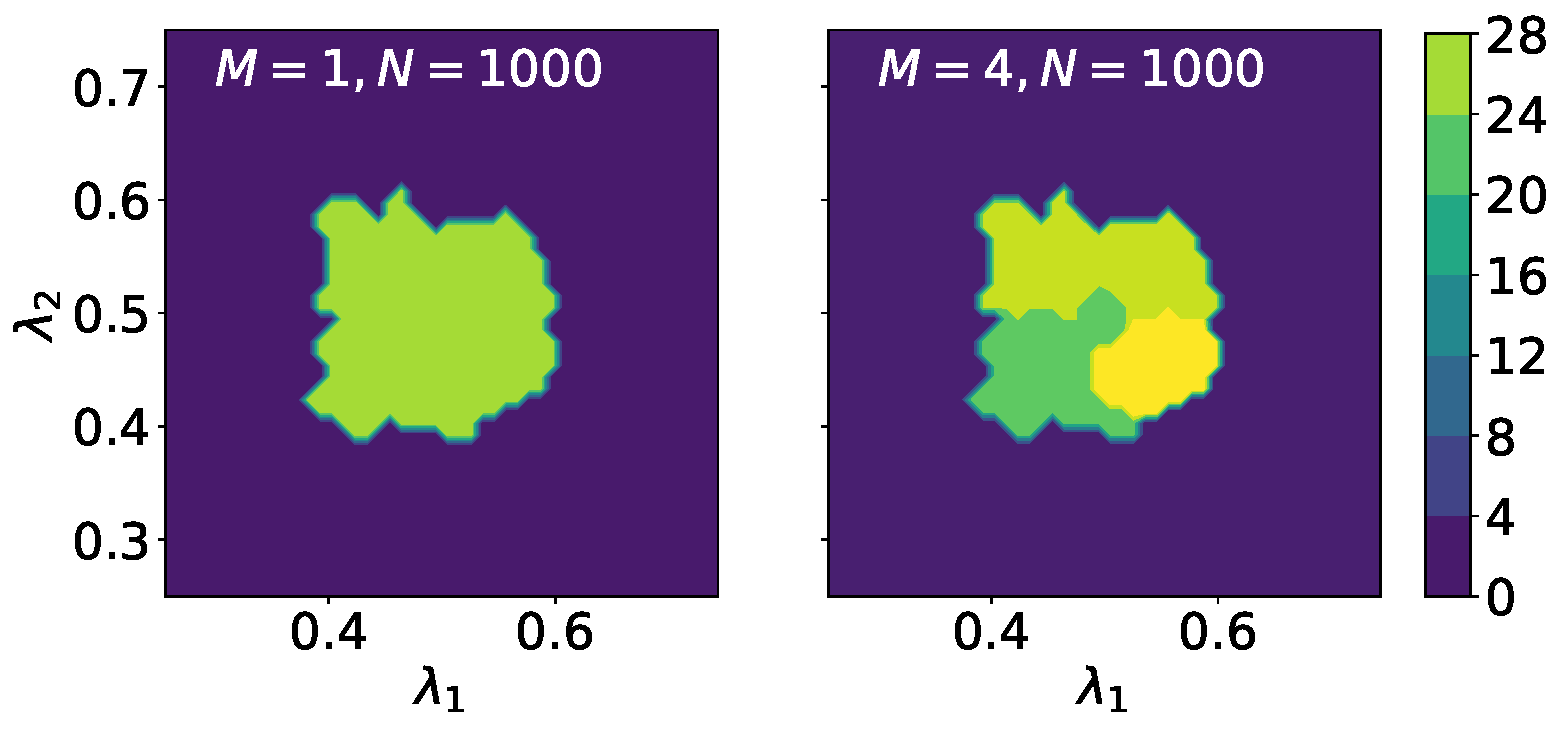
\includegraphics[width=\linewidth]{./examples/identity/set/M1-N1000_N1000-vs-M4-N1000_N1000.pdf}
\end{minipage}
\caption{
$\nsamps=1,000$ were used to discretize $\pspace$ and $\ndiscs=1, 4$ (left/right) were used to discretize $\dspace$.
TK
}
\label{fig:ex:identity_set_1E3}
\end{figure}
\begin{figure}[ht]
\begin{minipage}{.975\textwidth}
  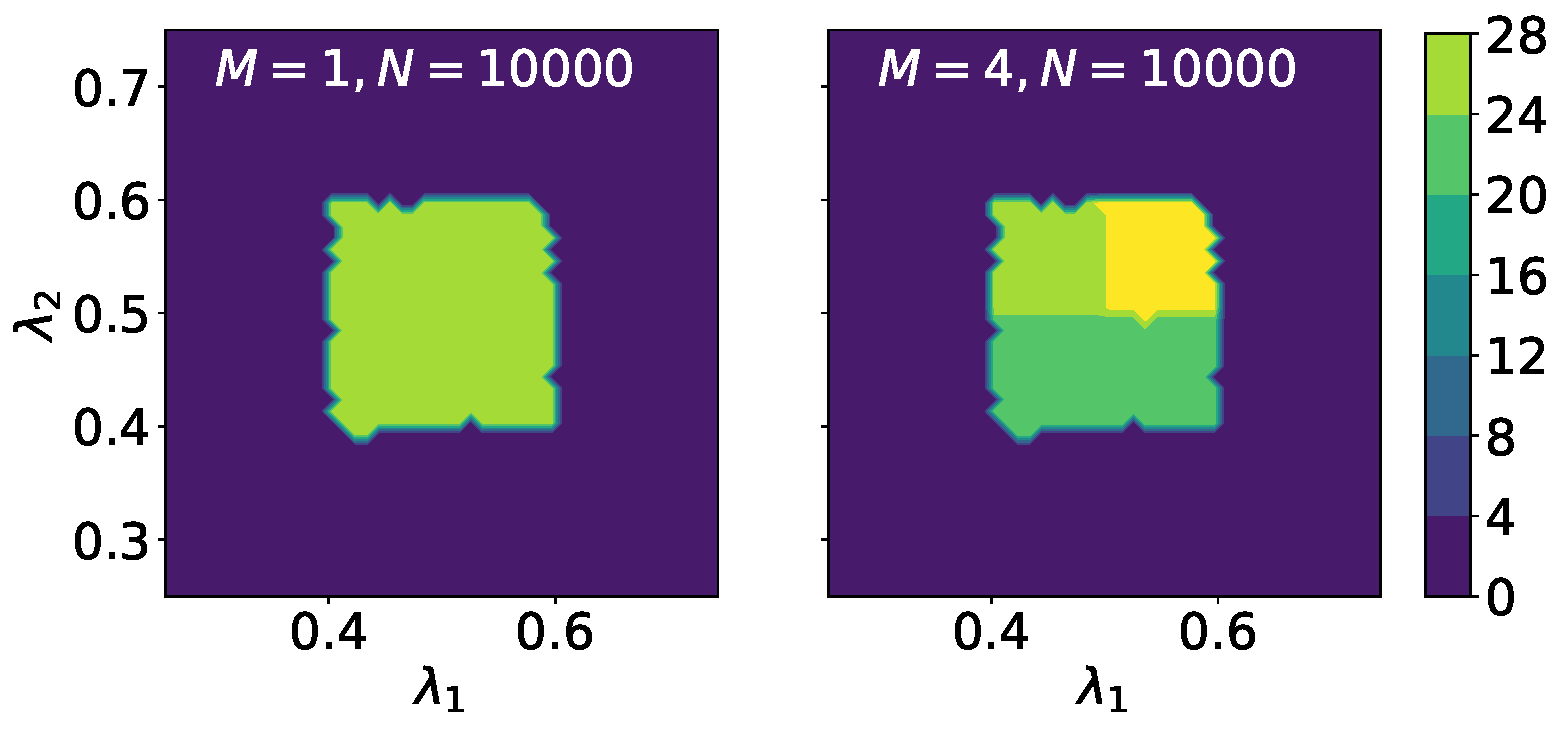
\includegraphics[width=\linewidth]{./examples/identity/set/M1-N10000_N10000-vs-M4-N10000_N10000.pdf}
\end{minipage}
\caption{
$\nsamps=10,000$ were used to discretize $\pspace$ and $\ndiscs=1, 4$ (left/right) were used to discretize $\dspace$.
TK
}
\label{fig:ex:identity_set_1E4}
\end{figure}
\FloatBarrier
